\chapter{REST API Proxy \\
  \small{\textit{-- Evan Ciok, Sophia DiCuffa, Carson McManus, Cindy Lee}}
  \index{Chapter!rest-api-proxy}
  \label{Chapter::RestApiProxy}}

\section{Forwarding API Requests}
When a REST API request is made to OpenTogetherTube, the request is first received by the load balancer
acting as the reverse proxy for API requests. The load balancer then selects one of the OTT monoliths based
on the current load balancing algorithm and forwards the request to the selected monolith. The monolith processes
the request and sends a response back to the load balancer acting as the reverse proxy. The load balancer then returns
the response to the client that made the original request.

\begin{figure}[!htb]
  \centering
  \scalebox{0.57}{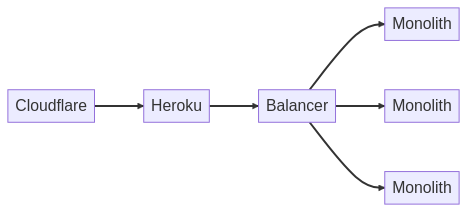
\includegraphics{Figures/api-balancer.png}}
  \caption{\label{Figure::api-balancer} API Balancer Flowchart.}
\end{figure}

\section{Forwarding Requests Credentials}

OpenTogetherTube platform uses tokens to authenticate and authorize users. When a user logs in, the
server generates a token that is stored in the browser's local storage and included in all subsequent requests made
by the user. The server verifies the token to ensure that the user is authenticated and has permission to access the
requested video stream. The token is used to look up the session information in Redis, which allows the server to
retrieve the user's permissions and session state.

\section{OpenAPI Endpoints Route Specification}

Table \ref{tbl:endpoints} shows each API endpoint and the route it will lead to. Additionally, it describes the function of each endpoint.


\begin{table}[htbp]
  \centering
  \caption{API Endpoints}
  \label{tbl:endpoints}
  \begin{tabular}{|c|l|c|p{5.5cm}|}
    \hline
    \textbf{Category}       & \textbf{Endpoint}               & \textbf{Methods}   & \textbf{Description}                                                                                              \\
    \hline
    \multirow{6}{*}{Room}   & /api/room/list                  & GET                & List open public rooms                                                                                            \\
    \cline{2-4}
                            & /api/room/{RoomName}/queue      & POST, DELETE       & Add one or more videos to the queue \newline Remove a video from the queue                                        \\
    \cline{2-4}
                            & /api/room/{RoomName}            & GET, PATCH, DELETE & Get room metadata \newline Change a room's settings or claim ownership of it \newline Unload the room from memory \\
    \cline{2-4}
                            & /api/room/generate              & POST               & Generate a new room                                                                                               \\
    \cline{2-4}
                            & /api/room/create                & POST               & Create a new room                                                                                                 \\
    \cline{2-4}
                            & /api/room/{RoomName}/vote       & POST, DELETE       & Add a vote for a video \newline Remove a vote for a video                                                         \\
    \hline
    \multirow{6}{*}{User}   & /api/user                       & GET                & Get the current user associated with the token                                                                    \\
    \cline{2-4}
                            & /api/user/auth/discord          & GET                & Authenticate user with Discord                                                                                    \\
    \cline{2-4}
                            & /api/user/auth/discord/callback & GET                & Callback for Discord authentication                                                                               \\
    \cline{2-4}
                            & /api/user/register              & POST               & Register a new user                                                                                               \\
    \cline{2-4}
                            & /api/user/login                 & POST               & Log in the current user                                                                                           \\
    \cline{2-4}
                            & /api/user/logout                & POST               & Log out the current user                                                                                          \\
    \hline
    \multirow{2}{*}{Data}   & /api/data/permissions           & GET                & Get roles and permissions data                                                                                    \\
    \cline{2-4}
                            & /api/data/previewAdd            & GET                & Get video preview data before adding it to the queue                                                              \\
    \hline
    \multirow{1}{*}{Dev}    & /api/dev/reset-rate-limit       & POST               & Reset rate limits (development mode only)                                                                         \\
    \hline
    \multirow{1}{*}{Auth}   & /api/auth/grant                 & GET                & Get an auth token                                                                                                 \\
    \cline{2-4}
                            & /api/auth/discord               & GET                & Authenticate with Discord                                                                                         \\
    \cline{2-4}
                            & /api/auth/discord/callback      & GET                & Callback for Discord authentication                                                                               \\
    \hline
    \multirow{2}{*}{Status} & /api/status                     & GET                & Get the status of the server                                                                                      \\
    \cline{2-4}
                            & /api/status/metrics             & GET                & Get server metrics for Prometheus                                                                                 \\
    \hline
  \end{tabular}
\end{table}

The routing between categories can be determined based on the relationships between the endpoints and the logical flow of the application. For example, endpoints within the "Room" category may have routes connecting to each other within the category, while endpoints in different categories may have separate routes.

API Specifications:
\begin{itemize}
  \item All /api/room/:roomName endpoints are routed to a specific monolith based on the :roomName parameter.
  \item /api/room/generate and /api/room/create are routed to the monolith with the least number of rooms.
  \item /api/room/list is a special case and will list rooms from all monoliths.
  \item /api/status and /api/status/metrics should not be forwarded as their responses are specific to each monolith and are only used for monitoring purposes.
  \item All other endpoints are stateless and can be routed to any available monolith.
\end{itemize}